\documentclass[11pt, oneside]{article}  	% use "amsart" instead of "article" for AMSLaTeX format
\usepackage{geometry}        		% See geometry.pdf to learn the layout options. There are lots.
\geometry{letterpaper}          		% ... or a4paper or a5paper or ... 
%\geometry{landscape}        		% Activate for rotated page geometry
%\usepackage[parfill]{parskip}  		% Activate to begin paragraphs with an empty line rather than an indent
\usepackage{graphicx}				% Use pdf, png, jpg, or eps§ with pdflatex; use eps in DVI mode
								% TeX will automatically convert eps --> pdf in pdflatex		
\usepackage{amssymb,amsmath}

\usepackage[most]{tcolorbox}
\usepackage[T1]{fontenc}
\usepackage[utf8]{inputenc}
\usepackage{natbib} 
\usepackage{alphabeta}

\title{ISTA (Iterative Shrinkage-Thresholding Algorithm) }
\author{M D Sacchi\,\footnote{emal: \texttt{msacchi@ualberta.ca}} }
\date{}							


\setlength{\parindent}{2em}
\setlength{\parskip}{1em}

\def\be{\vspace{0.0cm}\begin{equation}}
\def\ee{\vspace{0.0cm}\end{equation}}

\def\nin{\noindent}


\begin{document}
\maketitle
%\section{}
%\subsection{}

\section{Preliminaries}
When solving inverse problems and many signal processing problems, such as signal reconstruction, we often encounter the following 
\begin{align}
\hat{{\bf x }} &= \underset{{\bf x}}{\mbox{argmin }} \{ f({\bf x}) + \lambda\, g({\bf x}) \} \nonumber\\
      &= \underset{{\bf x}}{\mbox{argmin }} \{ \| {\bf A} {\bf x} - {\bf y} \|_2^2 + \lambda \| {\bf x} \|_1 \} \,.\label{l2_l1_problem}
\end{align}
Problems that can be written as equation \ref{l2_l1_problem} are often called $l_2-l_1$ problems. The statistical literature often calls the problem given by equation \ref{l2_l1_problem}  Basis Pursuit Denoising (BPDN). We are trying to find the minimum of $J$, the sum of two convex functions: the quadratic $l_2$ loss (misfit) and the $l_1$ regularization term. The main idea is to recover a sparse signal $\bf x$ from observations $\bf y$. These algorithms are used in Compressive Sensing to recover signals that have been compressed via a randomized sampling process  \citep{CS_Tutorial}. The problem is sometimes formulated as follows
\be
\mbox{min} \| {\bf x} \|_1 \quad \mbox{subject to } \| {\bf A} {\bf x} -{\bf y} \|_2^2 \le \delta 
 \label{l2_l1_problem_c}
\ee
\nin
Equation \ref{l2_l1_problem} is often called the unconstrained form of BPDN \citep{BPDN}. Conversely, equation \ref{l2_l1_problem_c} is
the constrained form of the problem. In what follows, we will adopt the unconstrained form where the single
tradeoff parameter $\lambda$ could be tuned to yield a sparse solution where $\| {\bf A} {\bf x} -{\bf y} \|_2^2 \le \delta $. In other words, we can find the constrained-form solution from the unconstrained problem. I prefer to use the unconstrained form of BPDN because it reminds me of classical Tikhonov regularization (the damped least-squares method), but with the critical difference that the $l_1$ regularization replaces the $l_2$-norm regularization norm. The unconstrained form of the problem also has a simple Bayesian
interpretation, whereas the constrained form (to my knowledge) does not.  


\subsection{ISTA solution}
I will start with the general problem where we minimize
the function $J= f({\bf x}) + \lambda g({\bf x})$ where $f$ and $g$ are convex functions

\be 
\hat{{\bf x }} = \underset{{\bf x}}{\mbox{argmin }} \{ f({\bf x}) + \lambda\, g({\bf x}) \} \label{general}
\ee
and then move on with the problem that involves minimizing the $l_2$ misfit in conjunction with an $l_1$ regularization term \citep{ISTA}.
The function $f({\bf x})$ can be approximated as follows 

\be f({\bf x}) \approx f({\bf x}_k) + \nabla f_k^T ({\bf x} - {\bf x}_k) + \frac{1}{2\eta} \| {\bf x} - {\bf x}_k\|_2^2
\label{approx} 
\ee
\nin
where $\nabla f_k^T$ is the gradient of $f({\bf x})$ at ${\bf x}_k$. Notice that if you take the derivative of the last equation and
equate it to zero; you will get the classical steepest descent step for updating the variable $\bf x$.
Hence, we can propose an algorithm that updates $\bf x$ in equation \ref{l2_l1_problem} via 
\be
{\bf x}_{k+1} = \underset{{\bf x}}{\mbox{argmin}} \, \{\, f({\bf x}_k) + {\nabla f}_k^T \,({\bf x} - {\bf x}_k) + \frac{1}{2\eta} \| {\bf x} - {\bf x}_k\|_2^2 +\lambda \,g({\bf x}) \,\}\,.
\ee
I can complete squares in the last expression and obtain the following 
\be
{\bf x}_{k+1} = \underset{{\bf x}}{\mbox{argmin}} \, \{\
  f({\bf x}_k)+ \frac{1}{2\eta} \| ({\bf x}- {\bf x}_k) + \eta {\nabla f}_k)\|_2^2- \frac{\eta}{2} {\nabla f}_k^T {\nabla f}_k + \lambda \,g({\bf x}) \}
  \,.
\ee
Now, I only keep terms that depend on the variable $\bf x$ (the others are constants that become zero after
differentiation)  

\be
{\bf x}_{k+1} = \underset{{\bf x}}{\mbox{argmin}} \, \{\
 \frac{1}{2\eta} \| {\bf x}- {\bf x}_k + \eta {\nabla f}_k)\|_2^2 + \lambda \,g({\bf x}) \}\,.
\ee
The last expression can be written as a denoising problem

\be
{\bf x}_{k+1} = \underset{{\bf x}}{\mbox{argmin}} \, \{\
 \frac{1}{2} \| ({\bf x} - {\bf u} )\|_2^2 + \eta \lambda \,g({\bf x}) \}\,, \label{prox1}
\ee
where ${\bf u} = {\bf x}_k - \eta {\nabla f}_k$. The above is a denoising problem where one tries to approximate the vector $
\bf u$ by $\bf x$ with an additional regularization $g({\bf x})$. The proximal operator gives the solution to equation \ref{prox1}. We generally choose $g$ such that the solution reduces to a univariate minimization problem with an analytical answer. Equation \ref{prox1} is written as follows
\begin{align}
{\bf x}_{k+1} =& \mbox{Prox}_{g,\lambda \eta} [{\bf u}]\\
           =& \mbox{Prox}_{g,\lambda \eta} [{\bf x}_{k} - \eta {\nabla f}_k]\,. \label{last} 
\end{align}

\subsection{Proximal operator for $g({\bf x}) = \|{\bf x}\|_1$}

The proximal operator for $g({\bf x}) = \| {\bf x} \|_1$ is named the soft-thresholding operator ${\cal S}_{\lambda \eta}$ and is the solution that
minimizes 
\be {\cal L} = \frac{1}{2} \| {\bf x} -{\bf v}\|_2^2 + a\, \|{\bf x}\|_1 = \frac{1}{2} \sum_i | x_i - v_i|^2 + a\, \sum_i | x_i |\,,\ee
where $a>0$. 
Setting $\frac{ \partial {\cal L}}{\partial x_k}=0$ leads to 

\be x_k-v_k + a\, \mbox{sign}(x_k)=0\,. \label{soft_1}\ee
The latter can be split into  
\begin{align}
v_k =& x_k - a \quad \mbox{if} \quad x_k<0\\
v_k = &x_k + a \quad \mbox{if} \quad x_k>0
\end{align}
The last expression needs to be inverted because we need $x_k$ as a function of $v_k$, an operation that
can be carried out graphically by first plotting the last expression $v_k=h_a(x_k)$ and then graphically (Figure 1) finding $x_k=h_a^{-1}(v_k)={\cal S}_{a}(v_k)$ which is
the soft-thresholding operator
\be
{\cal S}_{a}(v_k) =
\begin{cases}
  v_k - a& \quad  v_k > a\\
  0   &\quad   |v_k|\leq a  \\
  v_k + a& \quad v_k < -a
\end{cases} \label{soft}
\ee
 The operator
can be written in a more compact form as follows
\begin{equation}
{\cal S}_{a}(v_k) = \mbox{sign}( v_k )\, \mbox{max}( |v_k |-a, 0)\,.
\end{equation}


\subsection{Recap ISTA}
Let us go back to our original problem $f({\bf x}) = \| {\bf A } {\bf x} - {\bf y}\|_2^2$ and $g({\bf x}) = \| {\bf x} \|_1$. Then, according to equations \ref{last} and \ref{soft}
\begin{align}
{\bf x}_{k+1} = & {\cal S}_{\lambda \eta} [{\bf u}]\\
           = & {\cal S}_{\lambda \eta} [{\bf x}_{k} - \eta {\bf A}^T ({\bf A} {\bf x}_k -{\bf y}) ] \,. \label{last2} 
\end{align}
where the proximal operator (Soft thresholding, equation \ref{soft}) is applied element-wise.
The step length $\eta$  must satisfy $\eta< 1/\lambda_{max}$ where $\lambda_{max}$ is the maximum eigenvalue
of ${\bf A}^T {\bf A}$. The maximum eigenvalue of ${\bf A}^T{\bf A}$ can be iteratively found via the Power Method \citep{GoluVanl96}.

\begin{figure}[ht!]
  \centering
  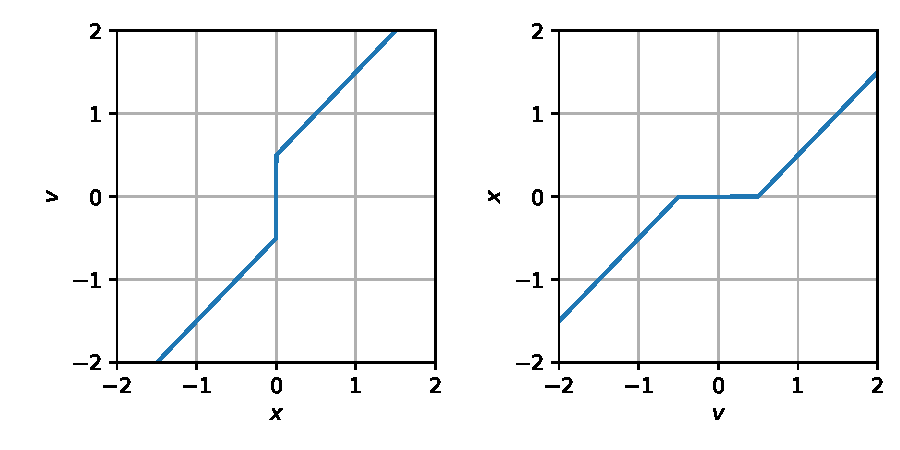
\includegraphics[width=0.9\textwidth]{soft.pdf} 
  \caption{Left is equation \ref{soft_1},  $v=h_a(x)$. Right is the soft thresholding operator $x={\cal S}_{a}(v)$ (equation  \ref{soft}), $a=0.5$. }
  \label{fig:0}
\end{figure}


\section{Example}
Figure \ref{fig:1} shows the inversion of a sparse sequence $\bf x$ that has been compressed via a random matrix 
$\bf A$. The compressed
data is given by ${\bf y} = {\bf A} {\bf x} + {\bf e}$ where $\bf y$ has 40 points. The original signal $\bf x$ has 150 points. This is an underdetermined problem, and we are exploiting the fact that $\bf x$ is sparse to recover it from
the measurement vector $\bf y$. I am comparing ISTA,  FISTA (Fast-ISTA) \citep{FISTA} and IRLS \citep{Sacchi}. Figure 2 provides
the convergence curves of these three algorithms. 

\begin{figure}[htbp]
  \centering
  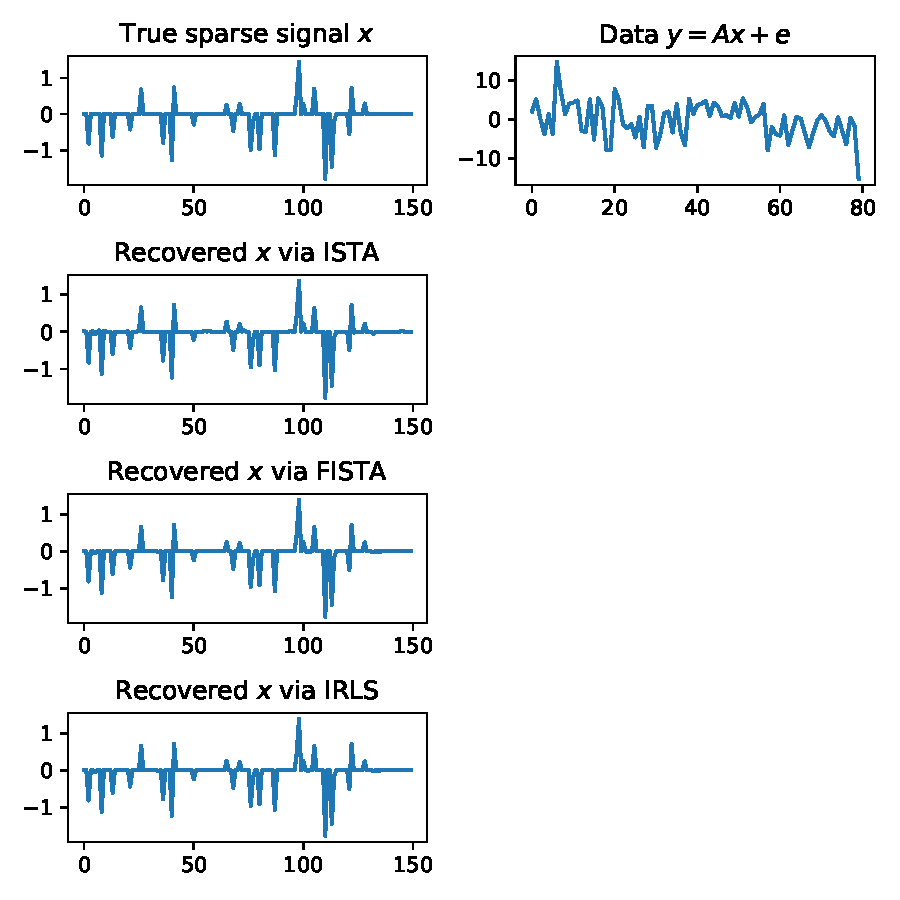
\includegraphics[width=0.9\textwidth]{comparison.pdf} 
  \caption{Inversions via ISTA, FISTA and IRLS.}
  \label{fig:1}
\end{figure}

\begin{figure}[htbp]
  \centering
  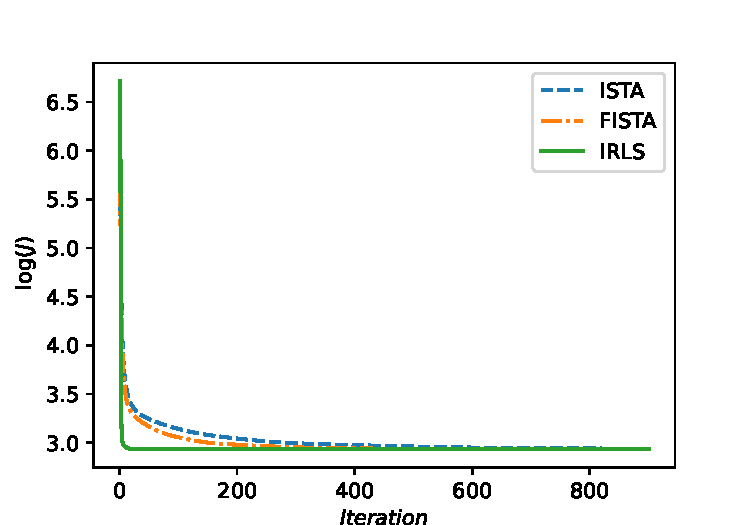
\includegraphics[width=0.9\textwidth]{convergence.pdf} 
  \caption{Convergence curves comparing ISTA, FISTA and IRLS.}
  \label{fig:e2}
\end{figure}
Notice that in the paper by \cite{Sacchi}, IRLS is used to solve the Fourier sparse reconstruction problem
via a Cauchy sparsity norm. A similar approach is used for multidimensional seismic signal reconstruction 
by \cite{Zwartjes}. The last two references are a good starting point for understanding ND seismic data reconstruction as it is used today by seismic data processing contractors. 
\begin{table}[htp]
\begin{center}
\begin{tabular}{|c|c|c|c|} \hline
  & ISTA & FISTA & IRLS\\ \hline
 $RMSE \times 100$ & 0.462& 0.178 & 0.198\\  \hline
\end{tabular}
\end{center}
\caption{Recovery error for the example in Figure  2 where $RMSE = \| {\bf x} - {\bf x}_{true} \|_2^2 / \| {\bf x}_{true} \|_2^2$.}
\label{default}
\end{table}

\section{ISTA Code}

\begin{tcolorbox}
\begin{verbatim}

function ISTA(A,y,Niter,λ)
# ISTA solver. Finds x that minimizes 
# J = 1/2||A x - y ||_2^2 + λ ||x||_1  
   
  Soft(x,alpha) = sign(x)*max(abs(x)-alpha, 0)

  N,M = size(A)
  e = Power_Iteration(A)  #
  η = 0.95/e
  
  x = zeros(Float64,M)
  
  J = zeros(Niter)
  for k = 1:Niter
    u = x .- η*A'*(A*x.-y)
    x = Soft.(u, η*λ)
    J[k] = 0.5*sum((A*x-y).^2) + λ*sum(abs.(x))
  end
    return x, J
end
\end{verbatim}
\end{tcolorbox}


\bibliographystyle{abbrvnat}
\bibliography{ref}

\end{document}  